\subsection{Расчет диаграммы транспортных возможностей неманевренного
самолета}
\label{sec:Расчет диаграммы транспортных возможностей неманевренного
самолета}
\pagestyle{fancy}
\fancyhf{}
\rhead{Дипломная работа}
\lhead{Расчёт транспортных возможностей}
\rfoot{\thepage}



\pagestyle{fancy}
\fancyhf{}
\rhead{Дипломная работа}
\lhead{Транспортные возможности самолёта}
\rfoot{\thepage}

Так как самолет Concorde предназначен для транспортировки пассажиров на различные расстояния, то необходимо знать его транспортные возможности, расчету которых и посвящен данный раздел. Ниже приведены формулы и соотношения, необходимые для проведения расчетов, а также пояснения к ним. 

\subsubsection{Расчетные формулы и соотношения}

Расчет ведется для трех режимов: 

\begin{enumerate}
    \item Полет с максимальной коммерческой нагрузкой
    \item Полет с максимальным запасом топлива
    \item Полет без коммерческой нагрузки ($m_\text{цн} = 0$) с максимальным запасом топлива
\end{enumerate}

\underline{Для режима №I} 

Дальность полета для данного режима определена в предыдущем подразделе (см. подраздел \ref{sec: Расчет характеристик крейсерского полета}) Относительная масса целевой нагрузки равна $\bar{m}_\text{цн}$ = 0,15. Для второго и третьего режимов дальность полета вычисляется по формуле $L = L_\text{наб} + L_\text{кр} + L_\text{сн}$. В целях упрощения расчетов принимается допущение, что дальности и расход топлива при наборе высоты ($L_\text{наб}$, $\bar{m}_{T_\text{наб}}$) и снижении ($L_\text{сн}$, $\bar{m}_{T_\text{сн}}$) для трех указанных режимов не изменяются. 

\underline{Для режима №II} 

Дальность полета для данного режима определяется по формуле
(\ref{eq:Дальность крейсерского полёта})
$$\bar{m}_\text{взл} = \frac{m_\text{взл}}{m_0}$$
Зная параметры $V$, $K$, $C_e$, соответствующих крейсерскому
полету, принимаются равными вычисленным в подразделе \ref{sec: Расчет характеристик крейсерского полета}. Взлетная масса самолета $\bar{m}_\text{взл}$ и относительная масса топлива, затраченного на крейсерский полёт, $\bar{m}_{T_\text{кр}}$ определяется следующим образом:

$$\bar{m}_\text{взл} = 1$$
\begin{equation}
    \label{eq:Относительная масса топлива, затраченного на крейсерский полет}
    \bar{m}_{T_\text{кр}} = \bar{m}_{T_{max}} - \bar{m}_{T_\text{наб}} -\bar{m}_{T_\text{сн}} -\bar{m}_{T_\text{анз}} - \bar{m}_{T_\text{пр}},
\end{equation}
где $\bar{m}_{T_{max}}$ -- максимальная масса топлива, заливаемого в баки

Целевую нагрузку для данного режима можно определить следующим образом
\begin{equation}
    \label{eq:Целевая нагрузка}
    \bar{m}_\text{цн} = 1 - \bar{m}_\text{пуст} - \bar{m}_{T_{max}}
\end{equation}

\underline{Для режима №III}

Для данного режима полета дальность вычисляется согласно формуле для режима №II, а масса топлива определяется согласно формуле (\ref{eq:Относительная масса топлива, затраченного на крейсерский полет}). Относительная взлетная масса для данного режима полета равна:

\begin{equation}
    \label{eq:Относительная взлетная масса}
    \bar{m}_\text{взл} = \bar{m}_\text{пуст} + \bar{m}_{T_{max}} 
\end{equation}

\subsubsection{Результаты расчета транспортных возможностей самолета}
\label{sec:Результаты расчета транспортных возможностей самолета}

Согласно формулам \ref{eq:Относительная масса топлива, затраченного на крейсерский полет}-\ref{eq:Относительная взлетная масса},\ref{eq:Дальность крейсерского полёта} и вышеизложенным комментариям, были
проведены следующие вычисления:

\textbf{Режим №I}

Полет с максимальной коммерческой нагрузкой 
$$L = 278,04 \text{ км} + 7610,74 \text{ км} + 314,16\text{ км} = 8202\text{ км}$$
$$m_\text{цн} = m_0 \cdot \bar{m}_\text{цн} = 0,2 \cdot 180000 \text{ кг}= 36 000 \text{ кг}$$ 

\textbf{Режим №II}

Полет с максимальным запасом топлива 
$$\bar{m}_{T_\text{кр}} = 0,42 - 0,018 - 0,0032 - 0,05 - 0,01 = 0,3388$$
$$m_\text{цн} = 1 - 0,5 - 0,42 = 0,08$$
$$L_\text{кр} = 11200\text{ км}$$
$$m_\text{цн} = m_0 \cdot \bar{m}_\text{цн} = 0,08 \cdot 180000 = 14400 \text{ кг}$$

\textbf{Режим №III}

Полет при максимальном запасе топлива без коммерческой нагрузки 
$$\bar{m}_{T_\text{кр}} = 0,42 - 0,018 - 0,018 - 0,0032 - 0,05 - 0,01 = 0,3388$$
$$\bar{m}_\text{взл} = 0,5 + 0,42 = 0,92$$

$$L_\text{кр} = 14238$$
$$m_\text{цн} = m_0 \cdot \bar{m}_\text{цн} = 0 \text{ кг}$$

Вычисленные дальность полета и целевая нагрузка для режимов 1-3 занесены в
таблицу \ref{tab:Дальность полета и целевая нагрузка для режимов 1-3} 

\begin{table}[H]
    \centering
    \caption{Дальность полета и целевая нагрузка для режимов 1-3}
    \begin{tabular}{|c|c|c|c|}
    \hline
        Режим & I & II & III  \\ \hline
        $L$, км & 6300 & 9954 & 11052,52 \\ \hline
        $m_\text{цн}$, кг & 36 000 & 14400 &0 \\ \hline
    \end{tabular}
    \label{tab:Дальность полета и целевая нагрузка для режимов 1-3}
\end{table}

По данным таблицы \ref{tab:Дальность полета и целевая нагрузка для режимов 1-3}  была построена диаграмма транспортных возможностей для самолета-прототипа Concorde

\begin{figure}[H]
    \center{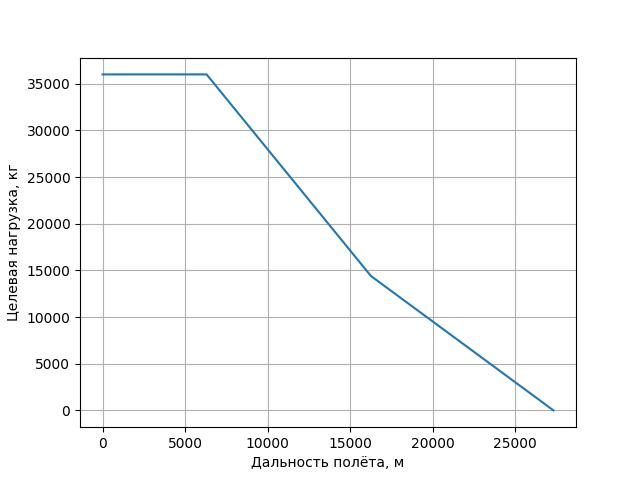
\includegraphics[width=\linewidth]{Оглавление/Part1/figures/Транспортные возможности.jpg}}
    \caption{Диаграмма транспортных возможностей неманевренного самолета Concorde (самолета –прототипа)}
    \label{fig:Диаграмма транспортных возможностей неманевренного самолета Concorde (самолета –прототипа)}
\end{figure}

\begin{center}
    Выводы:
\end{center}

Расчет транспортных возможностей показал следующие результаты:
\begin{enumerate}
    \item 8202 км -- дальность полета с максимальной коммерческой нагрузкой
    \item 11200 км -- дальность полета с максимальным запасом топлива
    \item 14238 км -- дальность полета при максимальном запасе топлива без
коммерческой нагрузки
\end{enumerate}

По данным результатам расчета самолет обладает хорошими транспортными
возможностями и может совершать полеты на значительные расстояния 

